\subsubsection{\texttt{RF-12}: rediseño del \textit{dashboard}}
\label{subsec:rf12}

El cuarto objetivo del Trabajo Fin de Grado es lograr un mayor nivel de intuitividad en la extensión, potenciando la interacción entre usuario y aplicación mediante elementos de la GUI que permitan, entre otras finalidades, que los usuarios ---y, específicamente en este caso, los docentes--- reciban la información proporcionada por la extensión de una forma legible, visual y clara.

Las versiones previas de \textit{VSCode4Teaching} incorporaban un \textit{dashboard} que cumplía su función adecuadamente, ya que mostraba el progreso de los estudiantes en tiempo real, aportando para cada uno datos como nombre y apellidos, nombre de usuario, el tiempo transcurrido desde la última modificación y el estado del ejercicio; pero que contaba con una estética poco desarrollada y que no mostraba métricas como, por ejemplo, la cantidad de alumnos que no habían comenzado aún el ejercicio o cuántos lo habían finalizado ya. Esta versión del \textit{dashboard} puede ser visualizada en la \referenciaFigura{fig:reqf12-1}.

\begin{figure}[ht]
    \centering
    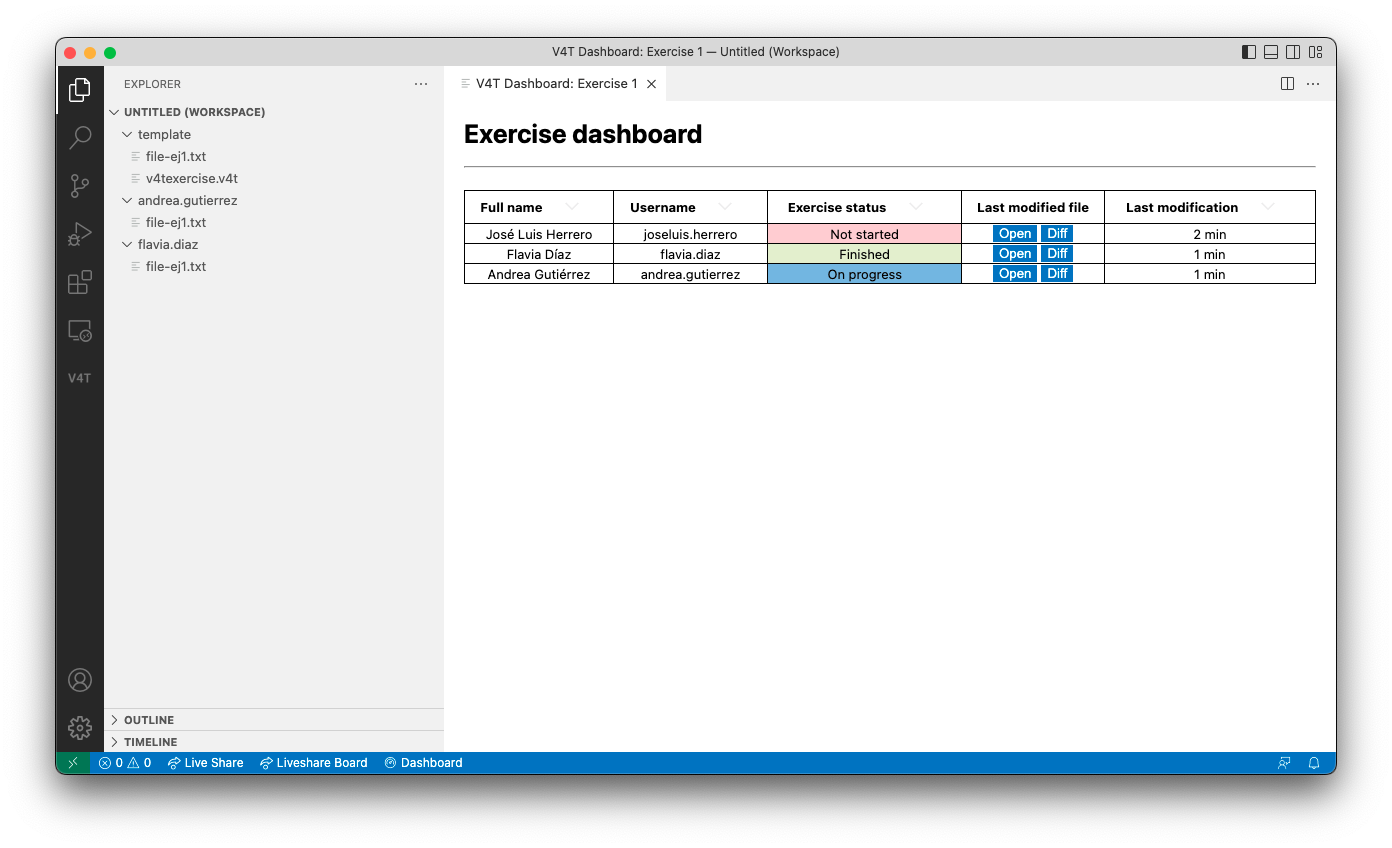
\includegraphics[width=0.925\textwidth]{imagenes/utilizadas/4-3-implementacion/rf12-1.png}
    \caption{Captura del \textit{dashboard} de \textit{VSCode4Teaching} previa a su modificación visual.}
    \label{fig:reqf12-1}
\end{figure}

\begin{figure}[ht]
    \centering
    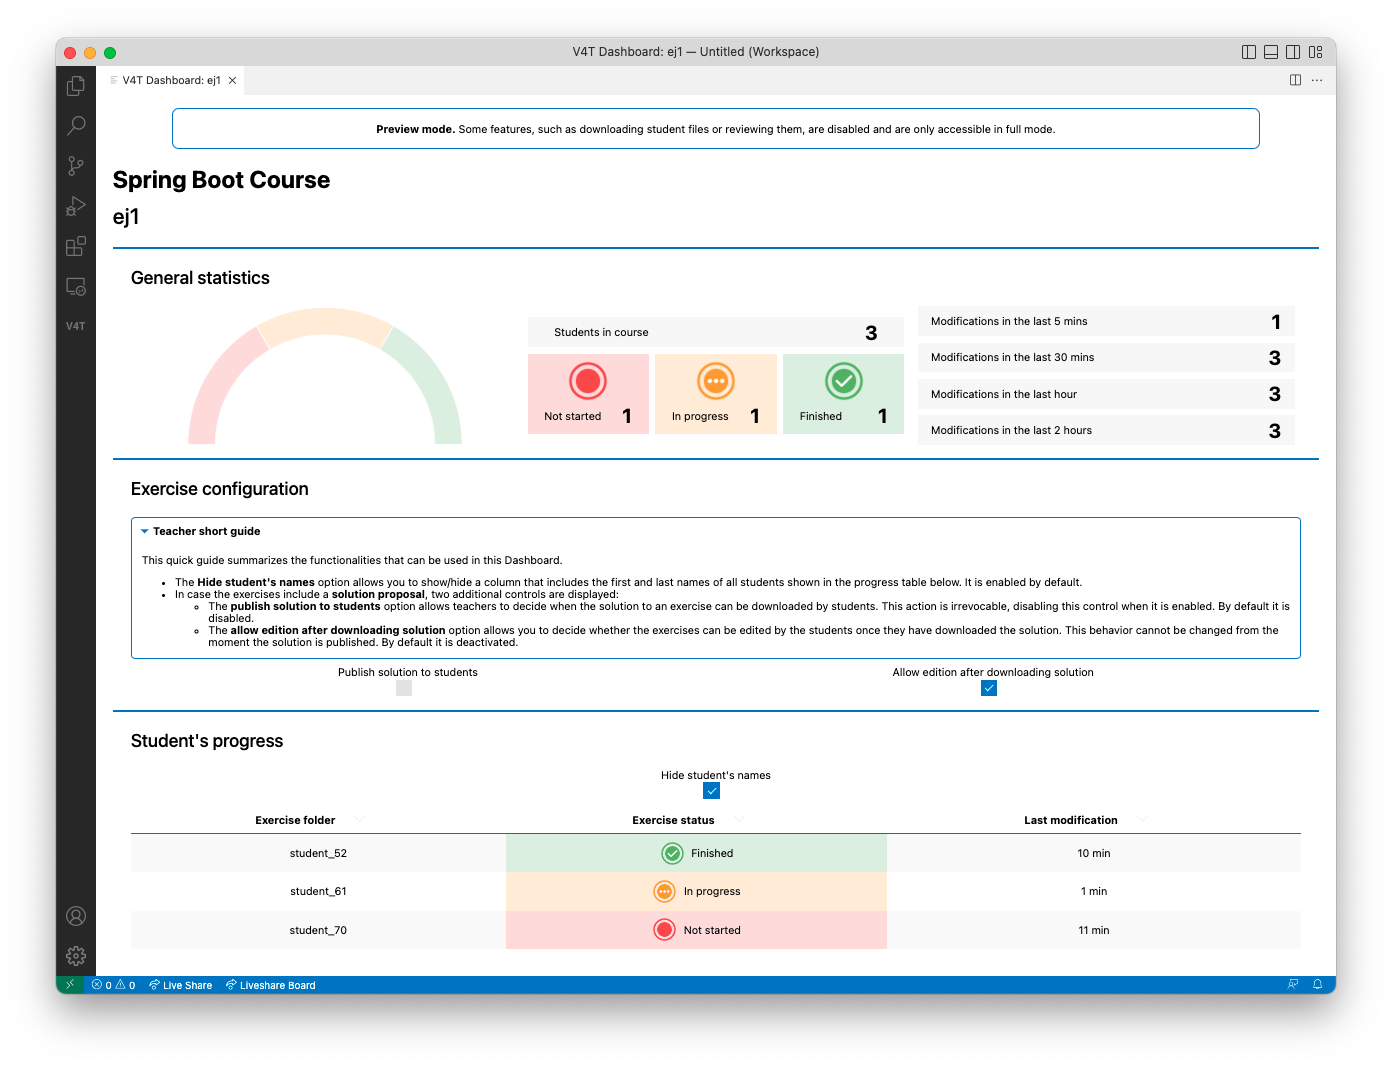
\includegraphics[width=0.925\textwidth]{imagenes/utilizadas/4-3-implementacion/rf12-2.png}
    \caption{Instantánea del \textit{dashboard} de \textit{VSCode4Teaching} tras su rediseño.}
    \label{fig:reqf12-2}
\end{figure}

Unificando el objetivo cuarto del proyecto \textit{VSCode4Teaching} ---véase \referenciaCapitulo{cap:objetivos}--- con la necesidad de generar una estética mejor y más funcional para el \textit{dashboard}, se ha ejecutado una labor de rediseño basada en tres ejes principales: la introducción de un gráfico semicircular que muestra la evolución del conjunto de estudiantes en la realización del ejercicio y la proporción de estudiantes que hay en cada uno de sus posibles estados, la introducción de nuevos parámetros estadísticos basados en el recuento de estudiantes presentes en cada uno de los estados del ejercicio y en la consideración del tiempo transcurrido en bloques de 5, 30, 60 y 120 minutos y la introducción de una guía de ayuda a docentes para explicar rápida y concisamente la funcionalidad de cada uno de los elementos de control y configuración presentes en el \textit{dashboard}.

Se introduce una instantánea del nuevo \textit{dashboard} en la \referenciaFigura{fig:reqf12-1} que, por comparación con la \referenciaFigura{fig:reqf12-2}, permite evidenciar la evolución introducida y la labor de rediseño ejecutada en una nueva visualización que cuenta con tres secciones claramente diferenciadas: una de estadísticas generales, en la que se introducen los nuevos elementos gráficos citados con anterioridad, otra de configuración en la que los docentes pueden acceder a la guía rápida y a la configuración sobre la solución ---en caso de haberla--- y una sección de progreso individual de los estudiantes, que muestra una tabla de estética mejorada con la información y funcionalidad que venía estando disponible en versiones anteriores.
